% !TeX spellcheck = en_US
\section{Video Composition}
\label{sec:240_videocomposition}
Live upload of video streams does not only offer the opportunity to apply adaptive video streaming but also another form of content adaptation: video composition.
Video composition applications offer the unique opportunity to improve the perceived quality and reduce generated data traffic in challenged networks~\cite{Arev2014,Saini2012,Shrestha2010,Wu2015}.
In contrast to adaptive video streaming, video composition achieves the quality increase and data traffic reduction by wisely selecting which video source should upload its video stream at a given time.
Out of a set of different close-by recording devices, only one (or a subset) is actively uploading its video.
Over time, different devices are allowed to upload, and the video composition algorithm ensures that exactly one composed video is created.
This section discusses the background on video composition and gives an overview of related systems conducting automatic composition for \ac{UGV}.
\subsection{Background on Video Composition}
Video composition is described as the "[...] arrangement of film properties, such as images [...], which create the total film [...]"~\cite[31]{Manchel1990}.
Many works, including this thesis, focus on the visual arrangement~\cite{Ward2003}, and especially the video shot selection.

\begin{figure}[tbh]
\centering

\includegraphics[width=\linewidth]{gfx/200_Background/RelatedWork_VideoComposition}
\caption[Central questions when switching between different video views]{Video composition: Central questions when switching between different video views.}
\label{fig:240_relatedworkvideocomposition}
\end{figure}

The video shot represents "[...] the smallest unit of visual information captured at one time by the camera that shows a certain action or event [...]"~\cite[2]{Bowen2013}.
It represents a consecutively recorded set of frames by a single camera.
If the position of the camera is stable during the recording of a shot, it is classified as a static shot, whereas camera movement during the recording classifies it as motion shot~\cite{Manchel1990}.
In a composed video, shots should be selected so that they do not distract viewers~\cite{Bowen2013}.
Essential is the concept of "content, then form", which expresses that a composed video shall express the semantics and action intended by the director~\cite{Manchel1990}.

Figure~\ref{fig:240_relatedworkvideocomposition} shows the concept of video composition that leverages different video sources to create a single quality-improved video.
For \ac{UGV}, a wise composition selects the best view at any given time.
The question as to which video view is the best at a given time is dependent on the perceived quality of individual sequences, the history of selected views and cinematographic rules.
An understanding of the influences on the perceived quality in composed videos is given in Section~\ref{sec:240_quality_composition}.
Also, video composition can reduce the generated data traffic in live video streaming scenarios as, ideally, only a single video source is used for video delivery.
\subsubsection{Video Views}
\label{sec:240_VideoViews}
It is assumed that the video composition aims at creating a video that leverages recordings capturing the same \ac{PoI}.
Different video sources thus capture different \emph{views} of the same \ac{PoI}.
These views differ regarding the recording position, thus, the distance and the angle to the \ac{PoI}.
The exact orientation of a device and the recording position can furthermore determine the shot type (often termed as shot size), which is known to have a specific impact on the perceived quality~\cite{Bowen2013,Manchel1990,Ward2003}.

A close-up is a magnified look at an object or a person, which contains very fine-granular visual information~\cite{Bowen2013}.
If a person is recorded, the close-up often represents the so-called "head shot", as the frame usually begins just below the chin.
It is often used to depict a character's emotions~\cite{Manchel1990}.

A medium shot reflects the common perception of a human in a close environment and is thus often used as the standard shot size~\cite{Bowen2013}. 
A person recorded in the medium shot is shown from the upper part of the legs and above.
The medium shot is usually recorded at a distance of 3 to 5 meters from the \ac{PoI}~\cite{Bowen2013}. 

In contrast, a medium-long shot includes the full person, possibly cutting off the feet.
It allows for retrieving and identifying clothing details.
At this distance, details on facial expressions and gestures are harder to see~\cite{Bowen2013}.

For capturing the whole scene in an inclusive manner, the long shot is used~\cite{Bowen2013}. 
Between the camera and the \ac{PoI} is a significant distance which allows framing the objects around a person.
However, details cannot be identified.

Different approaches~\cite{Arev2014,Saini2012} have shown that the automatic, exact framing (shot size selection) is not possible.
However, a good approximation is achieved when using the recording position in relation to the \ac{PoI} for determining the shot size  (without camera zoom).
\subsubsection{Quality of a Composed Video}
\label{sec:240_quality_composition}
An assumption of this work is that by leveraging different sources for constructing a composed video, the overall quality of the stream can be improved.
Related composition systems support this assumption, as video composition can increase the coverage of an event and ensures diversity compared to a single video stream~\cite{Arev2014,Saini2012,Shrestha2010,Wu2015}.
Also, by applying cinematographic knowledge, e.g., rules, the perceived quality of a composed video can be greater than the sum of the best parts of all single videos.
Cinematography grammar supports a told story by appropriately framing the action, proliferating emotions and strengthening the storyline.
\paragraph{Coverage and Continuity}
Single \ac{UGV} streams generated by \ac{MBS}s can be rather limited in duration.
From \ac{UGV} datasets, it is known that 90\% of the recording sessions are less than 10 minutes long, where the average is 3 minutes 54 seconds~\cite{Saini2013}.
These findings are supported by an analysis of the productive \ac{MBS} YouNow. 
The median is slightly higher than in the aforementioned dataset with approximately 16 minutes~\cite{Stohr2015}.

Video composition allows compensation for the fact that a single video track does not cover a full event. 
It does this by stitching content from different sources together into a composed video.
Ideally, all single video streams overlap to some extent and still allow the composed video to cover the duration of the full event.

In contrast to the completeness, continuity describes that the temporal sequence of a real-world event shall be kept in the composed video. 
Furthermore, the composition ensures that each segment of a video view should have a noticeable duration, so that viewers can perceive the view change.
\paragraph{Diversity of Video Recordings}
Different composition applications have shown that the major quality improvement in a composed video is the generated video view diversity~\cite{Arev2014,Saini2012,Shrestha2010,Wu2015}.
Diversity in video composition is defined as the "[...] use of a variety of views in the camera selection process to increase the information content in the generated video [...]"~\cite[7199]{Bano2015b}.
In professional productions, the diversity ensures that the perceived quality is enhanced~\cite{Bowen2013b,Zettl2016}.
Shrestha et al. support this concept for \ac{UGV} composition~\cite{Shrestha2010}.
For automatic composition, some general guidelines are proposed.
Saini et al. discuss that diversity should be guaranteed by inspecting the spatial and the temporal aspects of video views~\cite{Saini2012}.
Wu et al. add that diversity should not affect motion consistency, i.e., the direction and amount of motion in a frame~\cite{Wu2015}.
Ideally, static shots should be preferred and stitched to other static shots.

How video views should be switched is dependent on the content and genre of a composed video.
In the case of music videos, rapid switching between different views leads to specific composition styles, e.g., the \ac{MTV} composition style~\cite{Ward2003}.

Existing composition applications report that the diversity of video views promotes the attraction of the video and avoids boredom, but it must be ensured that view jumps are not too frequent~\cite{Arev2014}.
Professionally created video diversity is improved when cinematographic grammar rules are applied such as the "$180\degree$ rule" and the "$30\degree$ rule"~\cite{Arev2014,Wu2015}.
\paragraph{Cinematographic Rules}
Human directors learn guidelines on when a view switch shall happen and which views can be selected for composition from a cinematographic grammar~\cite{Dmytryk1984}.
A cinematographic or film grammar describes "[...] theories that describe visual forms [...] and their functions as they appear [...] during the projection of a film [...]"~\cite[96]{Manchel1990}. 
These rules shall be used to not distract viewers and support the storytelling of the video.
Dmytryk et al. gathered rules that describe how recording devices should be positioned~\cite{Dmytryk1984}.

\begin{figure}[tbh]
\centering
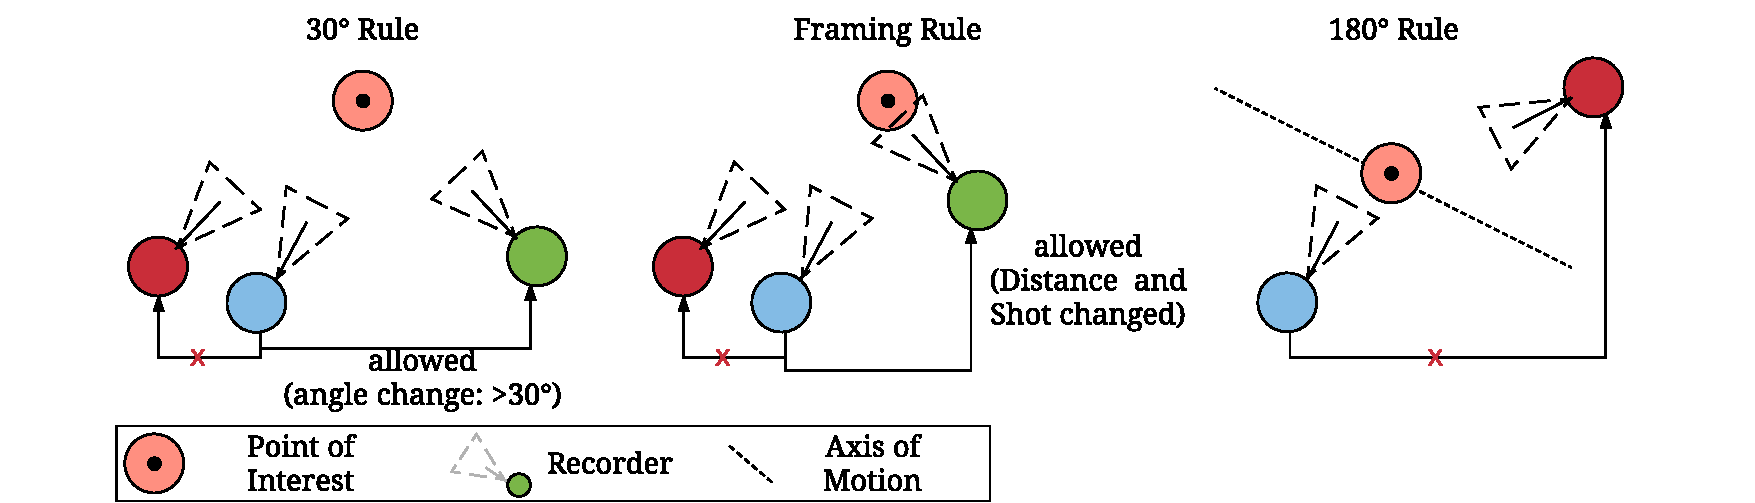
\includegraphics[width=\linewidth]{gfx/200_Background/RelatedWork_CinematographicRules}
\caption[Illustration of cinematographic rules]{Illustration of the cinematographic rules discussed in this thesis: "$30\degree$ rule", Framing rule and "$180\degree$ rule".}
\label{fig:240_relatedworkcinematographicrules}
\end{figure}

Most essential is the rule: "Content, then form".
It describes that the understanding of a scene being recorded helps to select a view.
The story and continuity of a composed video should be more important than other cinematographic rules.

Other examples of cinematographic rules are illustrated in Figure~\ref{fig:240_relatedworkcinematographicrules}.
The point in time when a switch between video shots takes place is named a cut.
\emph{Jump cuts} break the continuity in a video - either spatial or temporal.
Temporal jump cuts imply that between video shots no jump in time should be perceivable for the viewer.
This can be caused if the same subject is being recorded from the same or slightly varying recording positions.

Thus, when a video composition switches from one view to another, it needs to be ensured that the angle and distance of the two views are significantly different.
Cuts that preserve the temporal continuity but change the recording location should comply with two cinematographic rules.
The "$30\degree$ rule" should be respected regarding the recording angle.
It is applied if the same object or \ac{PoI} is recorded in two consecutive shots.
The rule recommends that between two consecutive video shots, there should be at least $30\degree$ of distance in the recording position.
At stable shot sizes, this rule is especially important.
The rule can be broken, i.e., the recording angle stays the same, but then the shot size needs to vary between two views~\cite{Proferes2005}.

The second rule discusses the \emph{framing}. From one shot to another, the framing of the two views should be different.
This may lead to a long shot following a medium shot in a composed video.

The switch should not conflict with the \emph{"$180\degree$ rule"}~\cite{Bowen2013b}.
It introduces the axis of action, which is of importance if any "[...] spatial (right-to-left or left-to-right) relationship between a character and another character or object [...]"~\cite[8]{Proferes2005} is recorded. 
This axis connects two or more major points of a view, e.g., interacting persons.
It describes the positions of objects, as well as the motion direction of objects or characters.
This axis should never be crossed, as a scene should never suffer from a direction reversal when switching between views.
Thus, a scene should not be captured from two opposite sides, as this may confuse the viewer.
Arev et al. have shown that such a switch from one side to another can be performed efficiently within a sequence of a few switches, but not within a single switch~\cite{Arev2014}.
For example, if objects leave a frame in a shot and return in a frame of the next shot, it needs to be ensured that they return to the same side (consistent screen direction or axis of action)~\cite{Proferes2005}.
\subsection{Existing Work on Automatic Video Composition}
In the remaining part of this section, existing approaches towards automatic video composition are discussed, which specifically deal with \ac{UGV}.
The approaches are classified reaching from a manual composition to automatic composition of \ac{UGV}.
\subsubsection{Categorizing Video Composition Applications}
Our discussion of related approaches is limited to composition algorithms for \ac{UGV} produced by smart mobile devices, e.g., retail mobile phones.
Professional productions or static camera recording issues are not discussed. 
The interested reader is referred to \cite{Lampi2010,Pozzer2009}.

A video composition as understood in the thesis has to be realized for live streaming scenarios in an automatic manner.
Thus, intuitive characteristics describing  existing video composition approaches address their capability to automatically (\emph{A}) compose video in real-time (\emph{RT}).

As the video recordings are provided by an \ac{MBS}, it is assessed if composition applications address that additional challenges arise such as synchronization of media streams, packet losses, and network-impaired delays.
This characteristic is termed \emph{network-awareness} (\emph{NW}).

Composition applications potentially receive a rather unlimited number of video streams which need to be processed.
Scalability (\emph{S}) assesses if complex processing can be conducted in a manner which allows distribution of tasks.

Furthermore, the video stream quality can vary over time. 
Three additional characteristics for classifying existing systems are if the composition system inspects the \emph{recording quality} (\emph{RQ}), \emph{video quality} (\emph{VQ}) and \emph{audio quality} (\emph{AQ}).
For these categories, a "$\circ$" represents that algorithms exist for detecting quality degradations, whereas a "+" represents approaches which quantify the perceived quality.
The quantification can be achieved either by using novel quality models created in subjective studies, or by leveraging established and validated objective quality metrics.

Essential for a high-quality composition is a suitable view diversity, which implies that views can be switched during composition.
The composition applications should mimic human composition, which ensures diversity over multiple switches. 
Thus, the composition algorithm should keep track of a history of selected views to ensure diversity (\emph{D}) in upcoming selections. 
If the algorithm considers both the view selection and duration, the system fulfills a suitable diversity (+).

The diversity can be influenced by both the consideration of different shot sizes and recording positions (\emph{RP}), complying with cinematographic rules (\emph{CR}) as well as the system being aware of the video content (\emph{CA}), i.e., different video genres require different composition styles.
  
The characteristics view selection (\emph{VS}) and cut point selection (\emph{CPS}) describe which underlying algorithms are used.
Algorithms are classified into human decision making (H), rule-based decision making (R), an optimization problem (O), and machine-learned decision making (ML).
Regarding the perceived quality of the composed video, human and machine-learned decision making (H,ML) are assumed to be the most beneficial~\cite{Saini2012}.

Which features are used in the decision making for VS and CPS are described with the feature characteristic (F).
Features are classified to be visual (V), audio (A), and auxiliary sensors (AS).  
\begin{table}
	\centering
	\caption[Comparison of existing video composition systems]{Overview of related work for automatic video composition applications. Features used for comparison include -- A: automatic composition; RT: real-time processing possible?; NW: network-aware; S: scalable; RQ: recording quality; VQ: video quality; AQ: audio quality; D: diverse composition; RP: recording position awareness; CR: compliance to cinematographic rules; CA: content-awareness; VS: algorithm used for view selection; CPS: algorithm used for cut point selection; F: features used for decision making. Values used are: +: implemented; $\circ$: compatible; - unsupported; V: visual; A: audio and AS: auxiliary sensors.}
	\begin{tabular}{lcccccccccccccc}
		\toprule[1.5pt]
		&  \textbf{A}  & \textbf{RT} & \textbf{NW} & \textbf{S} & \textbf{RQ} &\textbf{VQ} &\textbf{AQ} &\textbf{D} &\textbf{RP} & \textbf{CR} & \textbf{CA} &\textbf{VS} &\textbf{CPS} &\textbf{F}  \\ 
		\toprule[1.5pt]
		LACES~\cite{Freeman2014}  	& - & + & $\circ$ & -& - &-  & - & +& -& -& - & H & H & - \\
		WWM~\cite{Vihavainen2011} 	& $\circ$ & $\circ$ & - & - & - &-  & - & -& -& -& - & - & R & AS \\
		MotionHMM~\cite{Wang2008} 	& +  & - & - &- &-  &-  &-  &$\circ$ &- &- &-  &ML  &  -&V  \\
		LPC~\cite{Campanella2007} 	& + & - & - &  -& $\circ$ & $\circ$ & -& -&- & - &-  & R & R & V \\
		AMGS~\cite{Shrestha2010}    &  +& - & - &- &$\circ$& $\circ$ & - & $\circ$ & -& - & - & O & O &V  \\
		MoviMash~\cite{Saini2012} 	& + & - &-  & - & $\circ$ & $\circ$ & - & +& $\circ$& -& - & ML & R, ML & V  \\
		TComp~\cite{Arev2014} 		& + &-  &-  & -& $\circ$ & - & - & +& $\circ$& +& - & O & O &V  \\
		MoVieUp~\cite{Wu2015} 		& + &-  &-  &- &-  &$\circ$  & + & +& -& -& - & O  & O  & V,A  \\
		AudioCut~\cite{Roininen2016}& + & + & - & -&  -& - & $\circ$ & $\circ$ & - & -& - & - & ML & A  \\
		ViComp~\cite{Bano2015b} 	& + & - & - & - & $\circ$ & + & + &+ &- & - & - & R  & R & A,V \\
		SensorComp~\cite{Cricri2012} & + & + & - & - & $\circ$ & - & $\circ$ & - & - &- & - & R &  R&  AS,A\\
		\bottomrule[1.5pt]
	\end{tabular} 
	\label{tab:240_Related_Work}
\end{table}
\subsubsection{Human-supported Composition of UGV}
The manual composition system \ac{LACES} shall be representative for applications, which allow the composition of \ac{UGV}, but which do not offer automatic composition.
\ac{LACES}~\cite{Freeman2014} is a composition-supporting application for directors of live \ac{UGV}.
On a tablet, all recorded live video streams are gathered, and the director is allowed to manipulate the composed video.
It is well suited for in situ streaming scenarios, as the composed video can be provided as a live video stream.
Editing allows view and cut point selection, as well as frame editing and injection of non-live video.

The \ac{WWM} system~\cite{Freeman2014} offers an automatic, but not very sophisticated composition.
Switching between views is initiated by detecting panning using the compass of the recording devices. 
The view selection is not described so that a random selection is assumed.
An automatic composition is possible, but the provisioning and preprocessing of the video are done manually.
\subsubsection{Automatic Composition Application}
Wang et al.~\cite{Wang2008} proposed the first \ac{HMM}-based composition of video (MotionHMM).
While MotionHMM was not designed for \ac{UGV}, the model can be applied to it.
It learns view switching based on detected camera motion. 
A cut-point analysis is omitted.
\paragraph{Quality-aware Composition}
Campanella et al. introduced the assessment of camera shaking and motion, such as panning or tilting~\cite{Campanella2007}.
The proposed motion assessment algorithm is successful and reliable, and it is the basis for camera shake assessment in many composition applications~\cite{Bano2015b,Saini2012,Shrestha2010}.
The composition itself is very simplistic, solely relying on the detection of a camera shake and the video quality approximated by the brightness. 

Shrestha et al. propose a quality-aware video composition application for mobile phone recordings~\cite{Campanella2007}.
The \ac{AMGS} addresses recording quality assessment, e.g., inspecting camera shake.
Video composition is seen as an optimization problem that can be solved when investigating video quality, composition diversity, and cut-point suitability.
Diversity is interpreted so that each view needs to be shown at least once in the composition, even when its quality is low.
At the same time, the history of views solely considers the last video shot.
The optimization approach limits the application in live streaming scenarios, as it requires global knowledge of the full videos.
Furthermore, Shrestha et al.~\cite{Shrestha2007,Shrestha2010b,Shrestha2006} made contributions towards the synchronization of different video streams using audio fingerprinting or camera flash signals, which are used in \ac{AMGS}.

\paragraph{Recording Position-aware Video Composition}
MoviMash is a composition application designed by Saini et al. being evaluated for dance and music performances~\cite{Saini2012}.
MoviMash represents a sophisticated model as it learns compositions using a \ac{HMM}, after a video and recording quality assessment.
The used metrics for quality assessment are not validated with subjective studies and not reliant on established objective quality metrics.
As soon as a degradation is found within a view, the view is removed from further composition.
Yet, it does not offer content awareness. 
A single learned model is applied to any video genre, even though it has been trained with music video compositions only.
The resulting composed video shows a superior performance in comparison to quality-based algorithms, as, e.g., \ac{AMGS}~\cite{Shrestha2010}.

TComp was proposed by Arev et al. as no classical video composition, but as a video summarization application, as it integrates features for video condensing~\cite{Arev2014}. 
It is the only system that establishes precise location information on the basis of \ac{SfM} that focuses on head-mounted cameras.
It uses an optimization on the basis of a trellis-graph to ensure view diversity and cut-point detection.
Its computational overhead is one order of magnitude higher than required for real-time computation.
The composition follows basic cinematographic rules, such as the "$180\degree$ rule".

These composition applications are aware of the recording position, but no data is used to determine the quality of each recording position.
Rather, the positions are used for ensuring diversity~\cite{Saini2012} or applying cinematographic rules~\cite{Arev2014}.

\paragraph{Investigating the Audio Track of \ac{UGV}}
MoVieUp extends on MoviMash by adding an audio analysis and targeting specifically music recordings~\cite{Wu2015}.
It introduces the "less switching principle", which shows that in contrast to video, the audio track should not be diverse.
Furthermore, the audio track is assessed with respect to its quality and used for determining video view switches.
The quality assessment is based on the \ac{ITU} P.563 speech analysis algorithm~\cite{ITU-P563}.
An optimization problem is formulated and solved for the video selection.

Motivated by the intensive analysis of the audio track, AudioCut focuses solely on audio~\cite{Roininen2016}.
AudioCut is no complete video composition system, instead focusing on an audio-driven video cutting algorithm.
Thus, it does not determine how to select the best view; however, it is one of the few algorithms that does not analyze the visual parts of a video.
It focuses on concert recordings and shows that the cut point can be improved when inspecting the music meter and audio changes.
Transitions between audio recordings can be conducted smoothly when analyzing beat difference histograms.
The transitions are learned using an \ac{HMM}.

The design of ViComp focuses on the inspection of the audio track as well as some visual features~\cite{Bano2015b}.
The approach is clearly driven by audio analysis, but it also consists of a video analysis step using the subjectively validate no-reference image assessment metric \ac{BRISQUE}~\cite{Mittal2011}.
Besides image quality, camera shaking is analyzed as a quality-degrading factor (RQ).
View diversity is assumed to be sufficient if the last two video views are different from the current view.
The combined factor then determines which view is selected.
The cut point is determined using audio analysis, where a good cut is placed at a silent moment.
Silence is detected using the spectral entropy analysis of the audio track of each video.
When compared to MoviMash, this composition algorithm achieves a better quality in composition.	
\paragraph{Auxiliary Sensor-based Composition}
Cricri et al. introduced the first video composition application, which solely uses auxiliary sensor data to make composition decisions~\cite{Cricri2012}.
It uses the compass to calculate on the panning and tilting of the individual cameras, and to detect the \ac{PoI} by collaboratively filtering samples from different recording devices.
Also, the audio track of the video is inspected.
Whereas the combination allows for real-time composition of videos, it does not generate superior compositions in comparison to previously discussed work.
\subsection{Discussion}
Video composition is challenging when being realized as an automatic algorithm, as it has to consider a multitude of features and requires a significant processing overhead.
Existing applications evolved from human composition to automatic quality-aware systems.
Especially in the area of the quality, these algorithms neglect to consider the recording degradations or other quality effects such as the recording position.
Only MoviMash analyzes the recording position in order to ensure a suitable view diversity.
Their proposed approach neglects that selecting the next video view, and thus the recording position, has to comply with certain cinematographic rules.
Today, location sensors can help to easily identify the recording position and estimate the shot type.

Another major disadvantage of today's composition systems is the lack of real-time suitability. 
The inspection of visual features of high-quality video views is time-consuming.
Furthermore, the central approaches limit scalability.
All algorithms assume the video processing on a central server, without any discussion of the distribution of, e.g., quality assessment tasks.
Cricri et al. propose a centralized algorithm that instead focuses on auxiliary sensor data, e.g., from the accelerometer, to compose video in real-time~\cite{Cricri2012}.
The algorithm is not yet capable of achieving a quality similar to the videos composed by approaches using visual features.

The central challenges for upcoming composition algorithms are thus to combine visual, audio and auxiliary sensor-based features.
% -  -  -  -  -  -  -  -  -  -  -  -  -  -  -  -  -  -  -  -  -  -  -  -  -  -  -  -  -  -  -  -  -  -  -  -  - -
